\documentclass{jsarticle}

 \usepackage{ascmac}
 \usepackage{graphicx}
 \usepackage[dvipdfmx]{color}
 \usepackage{amssymb,amsmath,amsthm}
 \usepackage{graphics}
 \usepackage{fancybox, tcolorbox}
 \tcbuselibrary{raster,skins, breakable}
 \usepackage{nccmath}
 \usepackage{tikz}
 \usetikzlibrary{intersections, calc, cd}
 \usepackage{bm}
 \usepackage[italicdiff]{physics}
 \usepackage{titlesec}
 \usepackage{mathtools}
 \usepackage{enumerate}
 \usepackage{float}

 \numberwithin{equation}{section}
 \setcounter{tocdepth}{3}

\title{{光生物物理化学(物理パート) \\[2ex]\large 最終更新日: \today}}
\author{八木俊輔}
\date{}

\theoremstyle{definition}

\newcommand{\ave}[1]{\langle #1 \rangle}

\usepackage{fancyhdr}
\pagestyle{fancy}
    \lfoot{}
    \cfoot{\thepage}
    \rfoot{}

\begin{document}
\maketitle
\tableofcontents
\clearpage

\section{電磁波の反射と屈折}
これまでは一様な誘電体のなかでの電磁波の伝搬の様子を調べてきた.
ここでは,2つの異なる誘電体が,ある境界面で接しているときを考えよう.
このとき電磁波はその境界面で反射または屈折をすると考えられる.
誘電体のなかの平面波を
\begin{equation}
    \bm{A} (\bm{x}, t) = \frac{1}{i \omega} \bm{E}_0 \exp( i (\bm{k} \cdot \bm{x} - \omega (k) t) )
\end{equation}
とかいたとき,電場は
\begin{equation}
    \label{denba}
    \bm{E} (\bm{x}, t) = - \pdv{\bm{A} (\bm{x}, t)}{t} = \bm{E}_0 \exp( i (\bm{k} \cdot \bm{x} - \omega (k) t) )
\end{equation}
であたえられ,磁場は
\begin{equation}
    \label{ziba}
    \bm{B} (\bm{x}, t) = \curl{ \bm{A} (\bm{x}, t)} = \frac{\bm{k} \times \bm{E}_0}{\omega (k)} \exp( i (\bm{k} \cdot \bm{x} - \omega (k) t) )
\end{equation}
となる.ただし,$k := |\bm{k}|$ である.
そこで,(\ref{denba}), (\ref{ziba}) の平面波の境界面での反射または屈折を調べることにする.
そのためには,境界面上で電磁波が満たすべき境界条件を考えなければならない.\\
\quad 境界条件を決定するため,誘電体の中の自由電磁場の基本方程式系(\ref{fara})~(\ref{clom})を考える.
\begin{equation}
    \label{fara}
    \curl{ \bm{E} (\bm{x}, t) } + \pdv{\bm{B} (\bm{x}, t)}{t} = 0
\end{equation}
\begin{equation}
    \curl{ \bm{H} (\bm{x}, t) } - \pdv{\bm{D} (\bm{x}, t)}{t} = 0
\end{equation}
\begin{equation}
    \div{ \bm{B} (\bm{x}, t) } = 0
\end{equation}
\begin{equation}
    \label{clom}
    \div{ \bm{D} (\bm{x}, t) } = 0
\end{equation}
@@@\\
\quad 結局,境界条件はつぎのようにまとめられる.
\begin{tcolorbox}[colback=white, colframe=black]
    (i)  $\bm{B} (\bm{x}, t)$, $\bm{D} (\bm{x}, t)$ の法線成分は連続である.\\
    (ii)  $\bm{E} (\bm{x}, t)$, $\bm{H} (\bm{x}, t)$ の接線成分は連続である.
\end{tcolorbox}


さて,準備ができたので本論に入る.
入射平面波はつぎのようにかかれ,
\begin{equation}
    \label{nyusya1}
    \bm{E} (\bm{x}, t) = \bm{E}_0 \exp( i (\bm{k} \cdot \bm{x} - \omega (k) t) )
\end{equation}
\begin{equation}
    \label{nyusya2}
    \bm{B} (\bm{x}, t) = \frac{\bm{k} \times \bm{E}_0}{\omega (k)} \exp( i (\bm{k} \cdot \bm{x} - \omega (k) t) )
\end{equation}
反射波は,
\begin{equation}
    \bm{E'} (\bm{x}, t) = \bm{R}_0 \exp( i (\bm{k'} \cdot \bm{x} - \omega' (k') t) )
\end{equation}
\begin{equation}
    \bm{B'} (\bm{x}, t) = \frac{\bm{k'} \times \bm{R}_0}{\omega' (k')} \exp( i (\bm{k'} \cdot \bm{x} - \omega' (k') t) )
\end{equation}
また屈折波は,
\begin{equation}
    \bm{E''} (\bm{x}, t) = \bm{D}_0 \exp( i (\bm{k''} \cdot \bm{x} - \omega'' (k'') t) )
\end{equation}
\begin{equation}
    \bm{B''} (\bm{x}, t) = \frac{\bm{k''} \times \bm{D}_0}{\omega'' (k'')} \exp( i (\bm{k''} \cdot \bm{x} - \omega'' (k'') t) )
\end{equation}
と文字を設定する.\\
\quad ここで2つの誘電体の境界面を $z = 0$ の $x,y$ 平面上にとったとする.
すると,$z = 0$ にて境界条件(i), (ii)が要求される.
これらの条件は上の波動の各成分について線形な条件であるため,一般に
\begin{equation}
    A(x, y, z = 0, t) + B(x, y, z = 0, t) = C(x, y, z = 0, t)
\end{equation}
の形をしているため,
\begin{equation}
    \omega (k) = \omega' (k') = \omega'' (k'')
\end{equation}
\begin{equation}
    k_x = k_x' = k_x''
\end{equation}
\begin{equation}
    k_y = k_y' = k_y''    
\end{equation}
でなくてはならない.
すなわち,3つの平面波の振動数は相等しく,また3つの波数ベクトル $\bm{k}, \bm{k'}, \bm{k''}$ は同一平面内になくてはならない.\\
\quad そこでこれらのベクトルでつくられる平面内に $x$ 軸をとることにする.
すると,
\begin{equation}
    k_y = k_y' = k_y'' = 0
\end{equation}
となる.
いま入射平面波は直線的な偏りをしているものとして,振幅 $\bm{E}_0$ の $(x, z)$ 平面内の成分を $E_p$,$y$軸方向の成分を $E_s$ とかく.
ここでの $E$ の添え字はp偏光,s偏光を表すものである.\\
\quad ここでp偏光,s偏光についてコメントする.
p偏光のpはparallel,sはsenkrecht(ドイツ語)からきている.
p偏光は入射面に対して平行(parallel)に振動する偏光,s偏光は垂直に振動する偏光だと定義されており,図 \ref{henko} が分かりやすい.
\begin{figure}[H]
    \begin{center}
    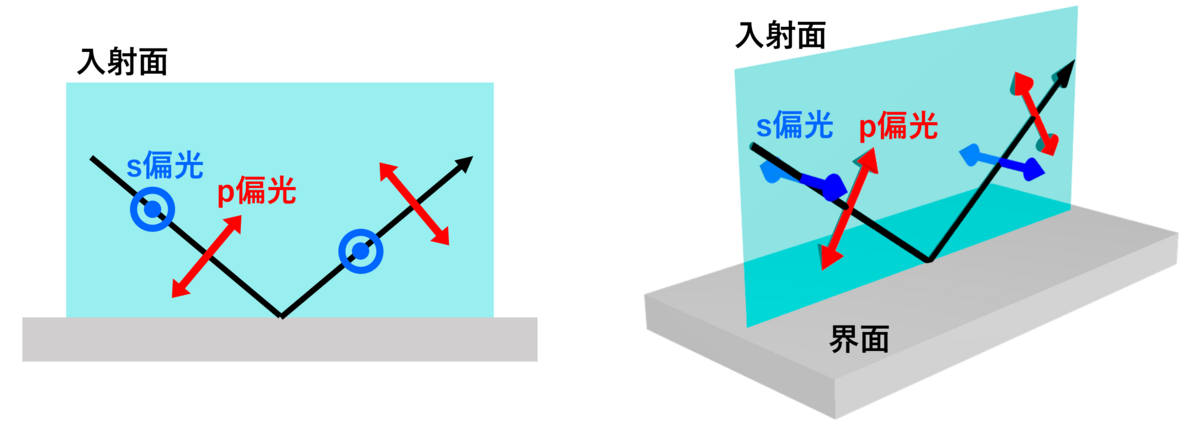
\includegraphics[width=10cm]{henko_ps.png}
    \end{center}
    \caption{p偏光とs偏光( https://casual-science-pedia.hatenablog.com/ より引用)}
    \label{henko}
\end{figure}
入射した光と反射した光により入射面が定まり,その面に含まれる成分がp偏光であって,垂直な成分がs偏光である.
今回のケースであれば,波数ベクトルについて $k_y = k_y' = k_y'' = 0$ よりy成分がs偏光となる.\\
\quad さて,図@のように改めて状況を設定する.
$\omega = v (\omega) k (\omega)$ に注意すれば,
\begin{equation}
    \bm{k} = (k_x, k_y, k_z) = \qty(\frac{\sin \varphi }{v_1 (\omega)} \omega, 0, \frac{\cos \varphi }{v_1 (\omega)} \omega)
\end{equation}
\begin{equation}
    \frac{\bm{k} \times \bm{E}_0}{\omega (k)} = \qty(-\frac{\cos \varphi }{v_1 (\omega)} E_s, \frac{1}{v_1 (\omega)}E_p, \frac{\sin \varphi }{v_1 (\omega)} E_s)
\end{equation}
となるため,\footnote{$v$の添え字はどちらの誘電体の中なのかを表している.} 入射平面波(式(\ref{nyusya1}), (\ref{nyusya2}))の成分は
\begin{equation}
    E_x = \cos \varphi E_p e^{-i \delta_1}, E_y = E_s e^{-i \delta_1}, E_z = - \sin \varphi E_p e^{-i \delta_1} 
\end{equation}
\begin{equation}
    B_x = -\frac{\cos \varphi }{v_1 (\omega)} E_s e^{-i \delta_1}, B_y = \frac{1}{v_1 (\omega)}E_p e^{-i \delta_1}, B_z = \frac{\sin \varphi }{v_1 (\omega)} E_s e^{-i \delta_1}
\end{equation}
とかかれる.ただし
\begin{equation}
    \delta_1 = \omega \qty( t - \frac{\sin \varphi \cdot x + \cos \varphi \cdot z}{v_1 (\omega)} )
\end{equation}
である.
同様にして反射波と屈折波についても書き下せる.
\begin{equation}
    E'_x = \cos \varphi' R_p e^{-i \delta'_1}, E'_y = R_s e^{-i \delta'_1}, E'_z = - \sin \varphi' R_p e^{-i \delta'_1} 
\end{equation}
\begin{equation}
    B'_x = -\frac{\cos \varphi' }{v_1 (\omega)} R_s e^{-i \delta'_1}, B'_y = \frac{1}{v_1 (\omega)}R_p e^{-i \delta'_1}, B'_z = \frac{\sin \varphi' }{v_1 (\omega)} R_s e^{-i \delta'_1}
\end{equation}
\begin{equation}
    E''_x = \cos \chi D_p e^{-i \delta_2}, E''_y = D_s e^{-i \delta_2}, E''_z = - \sin \chi D_p e^{-i \delta_2} 
\end{equation}
\begin{equation}
    B''_x = -\frac{\cos \chi }{v_2 (\omega)} D_s e^{-i \delta_2}, B''_y = \frac{1}{v_2 (\omega)}D_p e^{-i \delta_2}, B''_z = \frac{\sin \chi }{v_2 (\omega)} D_s e^{-i \delta_2}
\end{equation}
ただし
\begin{equation}
    \delta'_1 = \omega \qty( t - \frac{\sin \varphi' \cdot x + \cos \varphi' \cdot z}{v_1 (\omega)} )
\end{equation}
\begin{equation}
    \delta_2 = \omega \qty( t - \frac{\sin \chi \cdot x + \cos \chi \cdot z}{v_2 (\omega)} )
\end{equation}
である.\\
\quad 簡単のために,$\mu_1 = \mu_2 = \mu_0$ が普通の物質では成り立つことを用いる.
これにより境界条件を考えるときに $\bm{B}$ と $\bm{H}$ を区別する必要がなくなる.
境界条件(ii)より 
\begin{equation}
    E_x (x, z = 0, t) + E'_x (x, z = 0, t) = E''_x (x, z = 0, t)
\end{equation}
\begin{equation}
    E_y (x, z = 0, t) + E'_y (x, z = 0, t) = E''_y (x, z = 0, t)
\end{equation}
\begin{equation}
    B_x (x, z = 0, t) + B'_x (x, z = 0, t) = B''_x (x, z = 0, t)
\end{equation}
\begin{equation}
    B_y (x, z = 0, t) + B'_y (x, z = 0, t) = B''_y (x, z = 0, t)
\end{equation}

\end{document}
